\chapter{Evaluation}
\label{chapt:evaluation}

This chapter describes the evaluation of the two different implementation of the system architecture. In first architecture introduced more than one memcached instances at layer 2 as figure~\ref{fig:system_architecture} shows and in the second introduced more than one Social Network engines at layer 1.

In order to measure the response time(RT) the Apache JMeter application~\cite{jmeter_url} is used. The Apache JMeter is an open source benchmark designed to test functional behavior and  measure performance, targeting web applications. Notably, the RT measured by JMeter may not be the real one, because the JMeter measures the elapsed time from just before sending the request to just after the last response from server has been received. So, the time to render the web page to client web browser and the execution of JavaScript code is not measured. Because the time to render the web page and the execution of the JavaScript code is client limited and depending on client performance and which web browser is used, this time is not the case for the following performance stretching. Furthermore, the specific page, which is requested in the following performance testing, has not using any AJAX call, in order to not misguide the results. Therefore, the RT measures the time from just before JMeter sends the request to just after the last response, sent by the Social Network engine, is received. Between this measured time interval, the Social Network engine performs the following actions:
\begin{enumerate}[I]
\item The Social Network engine sends a request to CDO Client for the application execution model.
\item \label{l:1} The CDO Client forwards this request to CDO Server.
\item Afterwards CDO Server queries mysql repocitory of application models and executions, and finally gets the executions results.
\item CDO Server forwards back the results through CDO Client to Social Network Engine.
\item Furthermore, the Social Network engine sends queries to Social Network DB in order to get all the necessary Social features for this application page
\end{enumerate}

\section{Improving Performance with memcached}
\label{sec:eval_memcache}
By introducing a memcached node, the Social Networking engine first ask the memcached node if has the tuples that it wants. So the previous steps(\emph{I} to \emph{V}) is not necessary and if the memcached node has cached the values that the Social Network wants the loop through CDO CIient - CDO Server and the repositories is bypassed. 

The test performed with the following loads: (L1) ten users requests \emph{two} applications consecutively one hundred times, (L2) ten users requests \emph{four} applications consecutively one hundred times and (L3) ten users requests \emph{eight} applications consecutively one hundred times. Each application in the previous loads has ten execution rows. In this experiment we kept constant the following components of system: the Elgg front-end apache server, the Social network database, and the CDO server - client communication. In the system, increased the number of memcached nodes.
The figure~\ref{fig:rtavg} shows the  average, minimum and maximum response time (RT) in milliseconds with the following system configuration: (C1) no memcached node, (C2) one memcached node and (C3) two memcached nodes.

\begin{figure}[h]
	\caption{The average response time for all configurations.}
	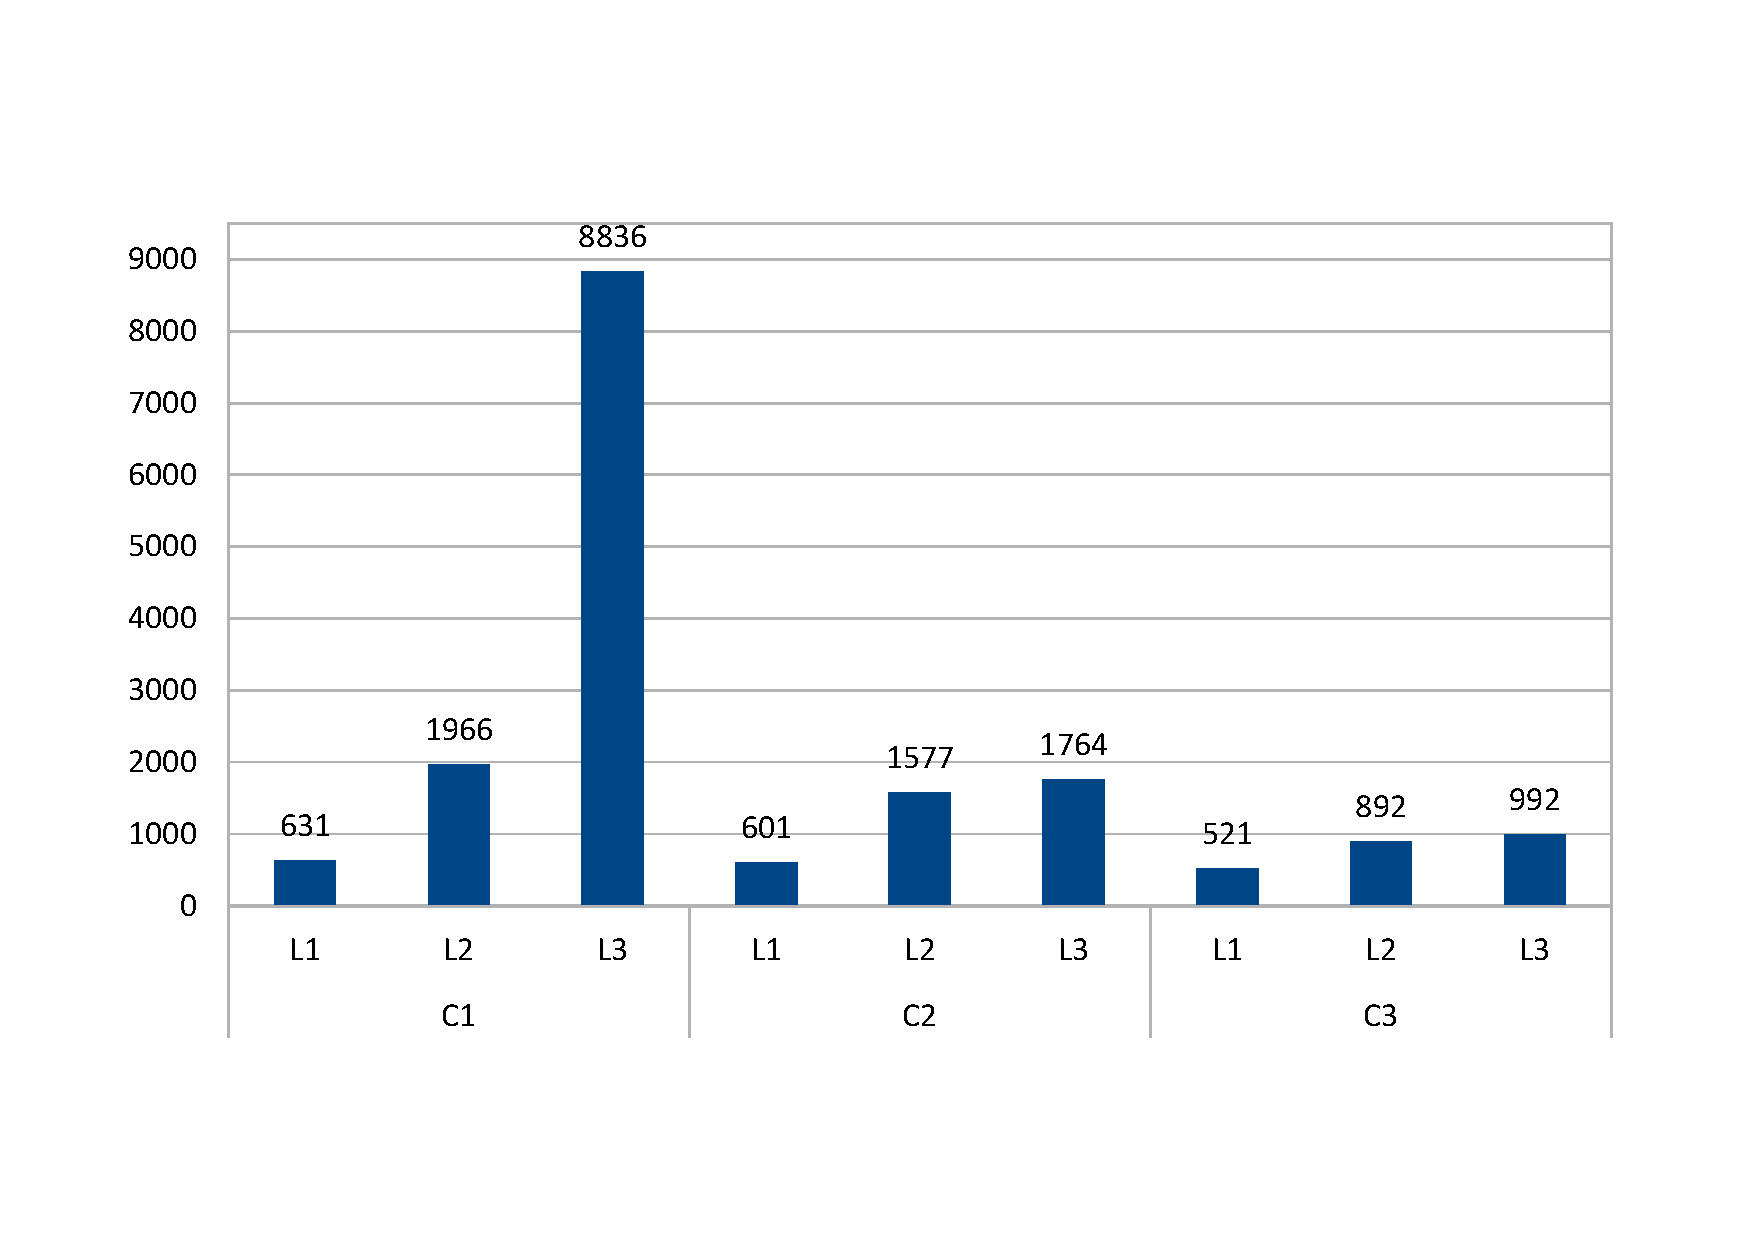
\includegraphics[width=0.6\textwidth,natwidth=200,natheight=150]{./fig/RTavg.pdf}
	\centering
	\label{fig:rtavg}
\end{figure}

As we going from C1 to C3 and specifically for L(oad) 3, the RT is reduced by 80,4\% at C2 and by 88,78\% at C3. As the figure~\ref{fig:rtavg} shows, at the first configuration C1, the L3 takes 8836 ms, a RT which is definitely prohibitive for web applications. Introducing more memcached nodes at C2 and C3 the RT is decreased dramatically 1764 ms at L2 and 992 ms at L3. Going from C1 to C2, the 80,4\% reduction of RT is due to introduction of memcached node and bypassed the steps I - V. Going from C2 to C3, the 43,77\% reduction of RT is due to more memcached nodes added, so more cpu cores were introduced to the architecture.

\begin{figure}[h]
	\caption{The average CPU utilization for all components.}
	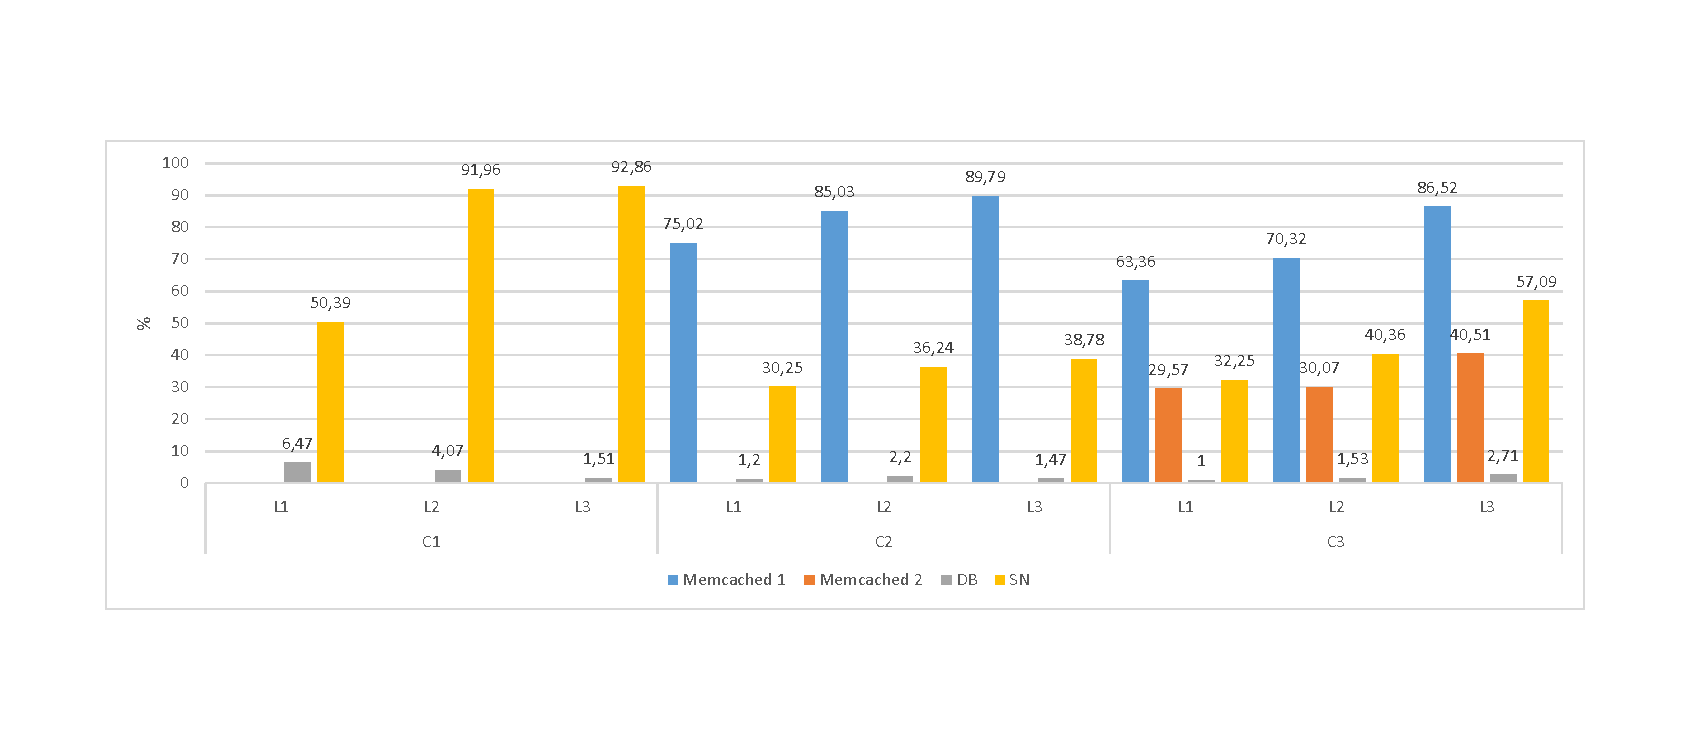
\includegraphics[width=1\textwidth,natwidth=200,natheight=150]{./fig/UsageAVG.pdf}
	\centering
	\label{fig:cpuavg}
\end{figure}

Furthermore, the CPU utilization is measured using the sysstat tool~\cite{sysstat_url}. We measure the CPU utilization for all the VMs running the experiment. The information about the VM resources is listed in table~\ref{table:vms_resources}. The Social Network engine with the CDO Client were running at t1.micro instance. The mysql (repositories) and the CDO Server were running at m1.xlarge. The average CPU utilazation is show in figure~\ref{fig:cpuavg}. At simple configuration C1, even in small load such as L1, the SN engine CPU utilization reached at 50,39\%. In the medium load L2 and big load L3 the SN engine is kneels down to 91,96\% and 92,86\%. This big consumption of CPU was due to all the initialization that Elgg Social Network engine have to do for each request and CDO Server - Client communication.

Moving from configuration C1 to C2, the CPU consumption went to memcached node. Thus, the Social Network engine was de-congested the RT improved. Although, for the big load L3 the memcached node was reach 89,79\%. Solving memcached CPU overhead, one more memcached node was added at configuration C3. This second memcached node was get the CPU overhead from one memcached node and the RT improved further again. At all loads at C3 the first memcached node has more CPU utilization from the second by an approximately factor of 2,2. The difference between the two memcached nodes appeared because the first node stores more popular key-value pairs than the other.

\begin{table}[]
\label{table:vms_resources}
\centering
\caption{VM resources}
\label{my-label}
\begin{tabular}{|l|l|}
\hline
 Component &  VM type \\ \hline
 SN engine, CDO client &  t1.micro \\ \hline
 memcached &  t1.micro \\ \hline
 repositories, CDO Server &  m1.xlarge \\ \hline
 jmeter &  m1.large \\ \hline
\end{tabular}
\end{table}

\section{Improving Performance with engine}
This section evaluates the horizontal scale of Social Network engine as described in~\ref{sec:engine_scale}. \ldots
%As mention in section ~\ref{sec:elgg_storage}, Social Network engine.